%------------------- Keys -------------------%
\subsection{Keys} \label{subsec:keys}

%------------------------------ I/O + constants + materials ------------------------------%
\subsubsection{Description}
This section gives information and calculations for the design of the keys on the shafts. The input is the applied torque and the output is the required length.
For this analysis, the shaft diameters (found in the shaft analysis) are considered as a constant. 
The key cross-sectional dimensions are chosen as a function of the shaft diameter: the width is a quarter of the diameter and the height is a third of the diameter. These values were chosen to balance the shear and compression acting on the key \cite{juvinall_fundamentals_2012}. A safety factor of at least 1.5 will be maintained, however it may be surpassed as the key length will be chosen to be the width of the part it is holding, for better stability.
The key material is selected to be the same as the shaft (marine grade stainless steel 316), however it is not cold treated and a lower yield strength (the minimum value) of $S_y=205 MPa$ is chosen. This value is selected to ensure that the keys would fail before the parts (pulleys, flange collars and hip plates), as the key is easier to replace.

%------------------------------ Stress Analysis ------------------------------%
\subsubsection{Stress Analysis and Free-Body Diagrams}
The free-body diagram in Figure \ref{fig:key_fbd} can be used to illustrate the forces acting on the key.

\begin{figure}
    \centering
    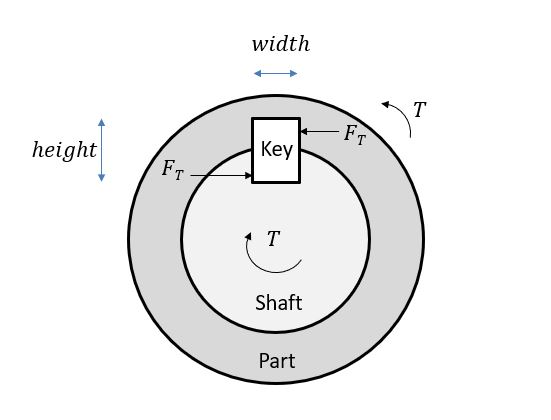
\includegraphics[width=0.6\textwidth]{4_Analysis/img/Key/key.JPG}
    \caption{Keys - Free-body diagram (cross-section of shaft)}
    \label{fig:key_fbd}
\end{figure}

Using the chosen cross-sectional ratios of the key (the width is a quarter of the diameter and the height is a third of the diameter), the following equations for the length of the key are found, as a function of the applied torque. The first is for the compressive force (crushing) acting on the key, and the second is for the shear of the key \cite{juvinall_fundamentals_2012}.

\begin{gather}
    L_{required}=\frac{12T}{S_yd^2} \label{eq:key_compression}
    \\
    L_{required}=\frac{8T}{0.58S_yd^2}=\frac{13.79T}{S_yd^2} \label{eq:key_shear}
\end{gather}

where $L_{required}$ is the required length of the key, $T$ it the torque applied on the key, $S_y$ is the yield strength of the key material and $d$ is the diameter of the shaft.
For the chosen geometry, the shear stress will always be slightly larger, thus Equation \ref{eq:key_shear} is used. The required key length must be no larger than the part it is holding. Safety factors are calculated to ensure 1.5 is reached.

The following is an example of the key dimensions calculation for the hip plate on the hip control shaft. First, the height and width are found based on chosen diameter ratios. Then, Equation \ref{eq:key_shear} is used to find the length. The applied torque is of 47440 Nmm, the shaft diameter at that point is 23.5 mm and the yield strength of the chosen material is 205 MPa. 

\begin{gather}
    height = d/3 = 23.5/3 =  7.83 mm
    \\
    width = d/4 = 23.5/4 = 5.88 mm
    \\
    L_{required}=\frac{13.79T}{S_yd^2}=\frac{13.79\times 47440 Nmm}{205 MPa\times (23.5 mm)^2}=5.78 mm
\end{gather}

As the width of the hip plate is of 10 mm, the key length is extended to $L=10mm$, thus we get the following safety factor:

\begin{equation}
    SF=\frac{L}{L_{required}}=\frac{10mm}{5.78mm}=1.73 > 1.5  \;\; Good!
\end{equation}

%------------------------------ Critical Review ------------------------------%
\subsubsection{Critical Review}
As the robot is a small application with relatively low torques, it would make sense that the size of the keys be relatively small as well. Thus, these results are representative.

%------------------------------ Parameterization ------------------------------%
\subsubsection{Parameterization}
This part will be parameterized by inputing the torque and shaft diameter and getting its required length. This length would then be increased to equal the width of the part it is holding, or the part itself will be made wider to ensure the key has an adequate length.